\documentclass[conference]{IEEEtran}

%%%%%%%%%%%%%%%%%%%%%%%%%%%%%%%%%%%%%%%%%%%%%%%%%%%%%%%%%%%%%%%%%%%%%%%%%%%%%%%%%%%%%%%%%%%%%%%%%%%%%%%%%%
\usepackage{amsmath,bm}
\usepackage{graphicx}

\def\MLine#1{\par\hspace*{-\leftmargin}\parbox{\textwidth}{\[#1\]}}
\graphicspath{ {./Images/} }
%%%%%%%%%%%%%%%%%%%%%%%%%%%%%%%%%%%%%%%%%%%%%%%%%%%%%%%%%%%%%%%%%%%%%%%%%%%%%%%%%%%%%%%%%%%%%%%%%%%%%%%%%%

%%%%%%%%%%%%%%%%%%%%%%%%%%%%%%%%%%%%%%%%%%%%%%%%%%%%%%%%%%%%%%%%%%%%%%%%%%%%%%%%%%%%%%%%%%%%%%%%%%%%%%%%%%
\begin{document}
%%%%%%%%%%%%%%%%%%%%%%%%%%%%%%%%%%%%%%%%%%%%%%%%%%%%%%%%%%%%%%%%%%%%%%%%%%%%%%%%%%%%%%%%%%%%%%%%%%%%%%%%%%
\title{Control systems}
\author{Xin Wang}
%%%%%%%%%%%%%%%%%%%%%%%%%%%%%%%%%%%%%%%%%%%%%%%%%%%%%%%%%%%%%%%%%%%%%%%%%%%%%%%%%%%%%%%%%%%%%%%%%%%%%%%%%%
\maketitle
%%%%%%%%%%%%%%%%%%%%%%%%%%%%%%%%%%%%%%%%%%%%%%%%%%%%%%%%%%%%%%%%%%%%%%%%%%%%%%%%%%%%%%%%%%%%%%%%%%%%%%%%%%
\section{Control system}
%%%%%%%%%%%%%%%%%%%%%%%%%%%%%%%%%%%%%%%%%%%%%%%%%%%%%%%%%%%%%%%%%%%%%%%%%%%%%%%%%%%%%%%%%%%%%%%%%%%%%%%%%%

\begin{figure} [h!]
    \centering
    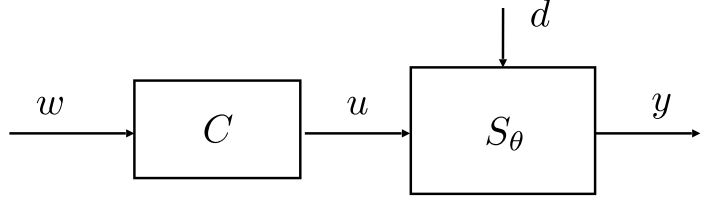
\includegraphics[scale=0.4]{Ex1.JPG}
\end{figure}
Notation:
\begin{itemize}
    \item $S_{\Theta}$: System to be controlled
    \item $C$: Controller
    \item $\Theta$: System parameters
    \item $y$: Controlled variable i.e. output
    \item $u$: Control variable (accessible)
    \item $d$: Disturbance factors
    \item $w$: Reference variable i.e. point 
\end{itemize}

%%%%%%%%%%%%%%%%%%%%%%%%%%%%%%%%%%%%%%%%%%%%%%%%%%%%%%%%%%%%%%%%%%%%%%%%%%%%%%%%%%%%%%%%%%%%%%%%%%%%%%%%%%
\subsection{Control system objective}

\begin{itemize}
    \item Act on $u$ to maintain $y \approx w$ in the presence of uncertainty
    \begin{align*}
        d  &= \bar{d} + \Delta d \\
        \Theta &= \bar{\Theta} + \Delta \Theta
    \end{align*}
    \begin{itemize}
        \item $\bar{d}$ and $\bar{\Theta}$ are known nominal values i.e. expected
        \item $\Delta d$ and $\Delta \Theta$ are uncertainties 
    \end{itemize}

    \item Uncertainty $\Delta d$ may have a known upper bound
    $$
        |\Delta d| < \bar{D}
    $$

\end{itemize}

%%%%%%%%%%%%%%%%%%%%%%%%%%%%%%%%%%%%%%%%%%%%%%%%%%%%%%%%%%%%%%%%%%%%%%%%%%%%%%%%%%%%%%%%%%%%%%%%%%%%%%%%%%
\section{Controller}
%%%%%%%%%%%%%%%%%%%%%%%%%%%%%%%%%%%%%%%%%%%%%%%%%%%%%%%%%%%%%%%%%%%%%%%%%%%%%%%%%%%%%%%%%%%%%%%%%%%%%%%%%%
\begin{itemize}
    \item Two kinds of controllers:
    \begin{itemize}
        \item Analog: Receives analog inputs and outputs analog 
        \item Digital: Processes digital sampled variables in computing devices
    \end{itemize}

    \item Conversion between two types requires: \textbf{ADC} and \textbf{DAC}
    \item Converters are synchronised via clock signal - period $T_s$
    \item Discrete-time variables can be expressed with time index
    $$
        t_k = kT_s \Rightarrow k
    $$
\end{itemize}

%%%%%%%%%%%%%%%%%%%%%%%%%%%%%%%%%%%%%%%%%%%%%%%%%%%%%%%%%%%%%%%%%%%%%%%%%%%%%%%%%%%%%%%%%%%%%%%%%%%%%%%%%%
\subsection{Digital control systems}

\begin{itemize}
    \item \textbf{Hybrid systems} - analog and digital variables 
\end{itemize}
\begin{figure} [h!]
    \centering
    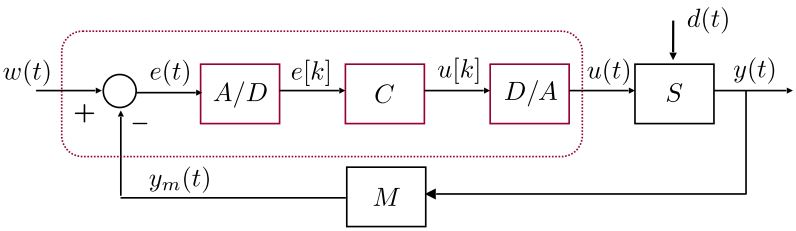
\includegraphics[scale=0.5]{Ex2.JPG}
\end{figure}

%%%%%%%%%%%%%%%%%%%%%%%%%%%%%%%%%%%%%%%%%%%%%%%%%%%%%%%%%%%%%%%%%%%%%%%%%%%%%%%%%%%%%%%%%%%%%%%%%%%%%%%%%%
\pagebreak
\section{Conversions}
%%%%%%%%%%%%%%%%%%%%%%%%%%%%%%%%%%%%%%%%%%%%%%%%%%%%%%%%%%%%%%%%%%%%%%%%%%%%%%%%%%%%%%%%%%%%%%%%%%%%%%%%%%

\begin{itemize}
    \item Types of variables:
    \begin{itemize}
        \item Continuous-time 
        \begin{figure} [h!]
            \centering
            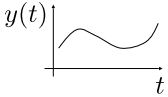
\includegraphics[scale=0.7]{Ex3.JPG}
        \end{figure}
        \item Piece-wise constants: Constant value between two sampling times
        \begin{figure} [h!]
            \centering
            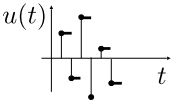
\includegraphics[scale=0.7]{Ex4.JPG}
        \end{figure}
        \item Discrete-time
        \begin{figure} [h!]
            \centering
            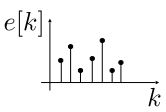
\includegraphics[scale=0.7]{Ex5.JPG}
        \end{figure} 
        \item Analog: Values change with continuity 
        \item Digital: Values are quantised
    \end{itemize}
\end{itemize}

%%%%%%%%%%%%%%%%%%%%%%%%%%%%%%%%%%%%%%%%%%%%%%%%%%%%%%%%%%%%%%%%%%%%%%%%%%%%%%%%%%%%%%%%%%%%%%%%%%%%%%%%%%
\subsection{A/D conversion}

\begin{figure} [h!]
    \centering
    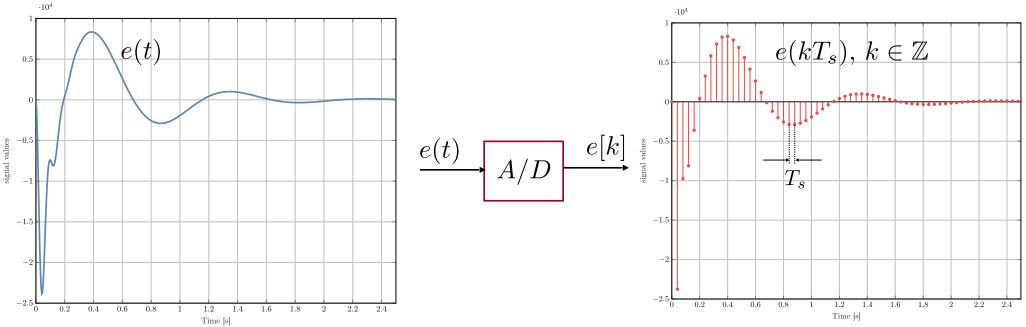
\includegraphics[scale=0.4]{Ex6.JPG}
\end{figure}

\begin{itemize}
    \item  Conversion uses the \textbf{sampling mechanism} 
    \begin{itemize}
        \item \textbf{Sampling frequency}: $f_s = \frac{1}{T_s}$
    \end{itemize}
    \item Implications:
    \begin{itemize}
        \item Loss of information 
        \item Quantisation of noise and distortion 
    \end{itemize}
\end{itemize}

\pagebreak
%%%%%%%%%%%%%%%%%%%%%%%%%%%%%%%%%%%%%%%%%%%%%%%%%%%%%%%%%%%%%%%%%%%%%%%%%%%%%%%%%%%%%%%%%%%%%%%%%%%%%%%%%%
\subsection{D/A conversion}

\begin{itemize}
    \item \textbf{Zero-order hold}: Stair-wise delayed approximation continuous-time function
\end{itemize}
\begin{figure} [h!]
    \centering
    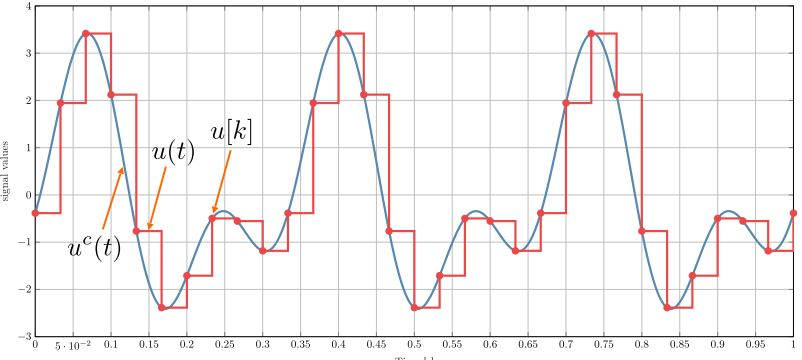
\includegraphics[scale=0.4]{Ex7.JPG}
\end{figure}

%%%%%%%%%%%%%%%%%%%%%%%%%%%%%%%%%%%%%%%%%%%%%%%%%%%%%%%%%%%%%%%%%%%%%%%%%%%%%%%%%%%%%%%%%%%%%%%%%%%%%%%%%%
\section{Digital discrete-time controller and control systems}

\begin{itemize}
    \item Controller is \textbf{computational algorithm}
\end{itemize}
\begin{figure} [h!]
    \centering
    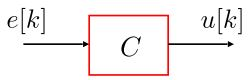
\includegraphics[scale=0.6]{Ex8.JPG}
\end{figure}
\begin{itemize}
    \item \textbf{Temporisation} i.e. delay
    \item Controller computation time should satisfy: $\Delta < T_s$ 
\end{itemize}
\begin{figure} [h!]
    \centering
    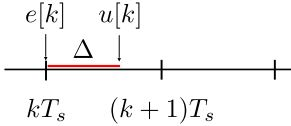
\includegraphics[scale=0.6]{Ex9.JPG}
\end{figure}

%%%%%%%%%%%%%%%%%%%%%%%%%%%%%%%%%%%%%%%%%%%%%%%%%%%%%%%%%%%%%%%%%%%%%%%%%%%%%%%%%%%%%%%%%%%%%%%%%%%%%%%%%%
\subsection{Control System}

\begin{itemize}
    \item \textbf{Error variable}: $e(t) = w(t) - y(t)$
    \item General requirements:
    \begin{itemize}
        \item \textbf{Static precision}: $y(t) \approx w(t)$ or $e(t) = 0$
        \item \textbf{Dynamic precision}: 
        \begin{itemize}
            \item Quick enough response time 
            \item Dampens possible oscillations 
            \item Able to track varying variables $w(t)$
        \end{itemize}
        \item Insensitive to disturbances i.e. reject $d(t)$
        \item Robust: Above condition hold for unknown system parameters
    \end{itemize}
\end{itemize}



%%%%%%%%%%%%%%%%%%%%%%%%%%%%%%%%%%%%%%%%%%%%%%%%%%%%%%%%%%%%%%%%%%%%%%%%%%%%%%%%%%%%%%%%%%%%%%%%%%%%%%%%%%
\end{document}
